\documentclass{article}
\usepackage{algorithmicx}
\usepackage{algpseudocode}
\usepackage{graphicx}

\begin{document}
{\noindent \Huge Problema a resolver:}
\newline \newline  El problema esta dado por la siguiente situaci\'on: nos encontramos en un extremo de un puente (afuera de \'el) y queremos llegar al otro extremo, bajo ciertas circunstancias y, si es posible hacer esto, hacerlo de la "mejor manera" (mas adelante se detallar\'a qu\'e significa esto y por qu\'e podr\'ia no ser posible atravesar el puente). El puente est\'a hecho con una cantidad \textit{n} de tablones seguidos y, algunos de ellos pueden estar rotos. Cuando esto suceda, vamos a querer saltar estos tablones rotos al atravesar el puente, pisando siempre tablones sanos cuando estemos avanzando.\newline
Tenemos una cantidad fija tablones seguidos que podemos saltar, la denominaremos \textit{c}, as\'i podemos ver que, si el puente tiene, en alg\'un momento, una cantidad \textit{$k > c$} de tablones rotos \textbf{seguidos}, entonces claramente no tendremos manera de atravesarlo ya que, intuitivamente, podemos pensar que, en el mejor de los casos (donde mejor significa estar lo m\'as alejados posibles del comienzo del puente) podr\'iamos estar en el tablon sano anterior (anterior inmediato) al primero de esos \textit{k} tablones rotos y, a\'un as\'i no podr\'iamos atravesar el puente ya que no podemos saltar m\'as de \textit{c} tablones seguidos, por lo tanto en cualquier otro caso (donde nos encontr\'aramos en un tabl\'on anterior al anterior inmediato del primero de los \textit{k} rotos por ejemplo), estar\'iamos en una situaci\'on similar porque eventualmente llegar\'iamos al tabl\'on sano que es el anterior inmediato al primero de los \textit{k} y quedar\'iamos estancados de la misma manera.
\newline En el caso en el que no se de la situaci\'on descripta anteriormente (es decir, en el caso en el cual s\'i podamos atravesar el puente), vamos a querer dar la menor cantidad de saltos (la "mejor manera").
\newline \newline Presentamos algunos ejemplos graficos junto a sus soluciones y las secuencias que lo representan. Los circulos con el A y el B determinan el punto de partida y el punto de llegada, ambos fuera del puente. Los tablones rotos est\'an pintados de negro.

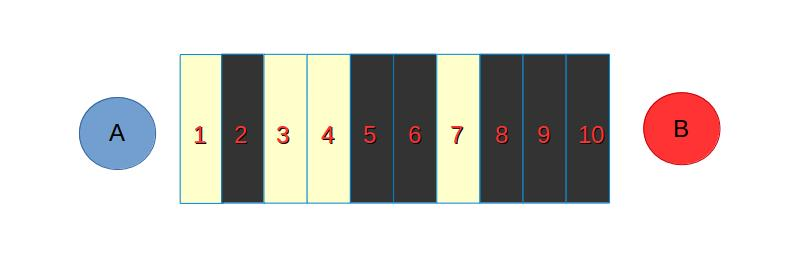
\includegraphics[width=\textwidth,height=\textheight,keepaspectratio
]{ejemplopuente1.jpg}
\begin {flushleft}
En este ejemplo, \textit{$n = 10$} y el puente se escribe como 10 c 0 1 0 0 1 1 0 1 1 1.
\newline Si \textit{$c = 3$}, entonces la soluci\'on est\'a dada por caer en los tablones 4 7 11. Notar que en realidad no existe un trabl\'on numerado con el 11, pero cuando exista una soluci\'on, para indicar que llegamos al punto de llegada, diremos que saltamos a un tabl\'on mayor estricto que la cantidad de tablones del puente (o sea, que estamos efectivamente fuera del puente).
Si tuvieramos el mismo puente pero con \textit{$n = 2$}, claramente no existir\'ia una soluci\'on ya que, si bien podr\'iamos llegar al tabl\'on 7 sin problemas, una vez ah\'i no tendr\'iamos manera de saltar el 8, 9 y 10 que est\'an rotos.\end {flushleft}
\vspace{1cm}
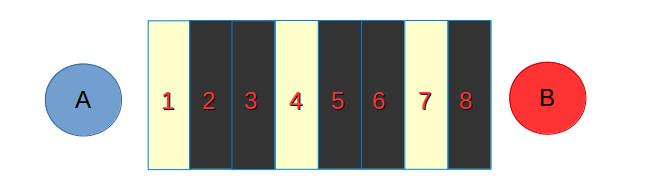
\includegraphics[width=\textwidth,height=\textheight,keepaspectratio
]{ejemplopuente2.jpg}
\begin {flushleft}Este otro puente se representa como 8 c 0 1 1 0 1 1 0 1.
\newline Si \textit{$c = 2$} entonces la soluci\'on es 1 4 7 9.
\newline Si \textit{$c = 1$} entonces no habr\'ia soluci\'on ya que hay 2 tablones rotos seguidos (esto ocurre dos veces en este caso particular pero con que ocurra una ya no hay soluci\'on posible).
\newline Si \textit{$c = 3$} la soluci\'on es  4 7 9.
\end {flushleft}

\vspace{1cm}
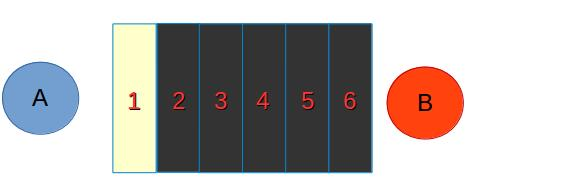
\includegraphics[width=\textwidth,height=\textheight,keepaspectratio
]{ejemplopuentes3.jpg}
\begin {flushleft}
Finalmente introducimos este ultimo ejemplo del puente 6 c 0 1 1 1 1 1.
Siguiendo la misma l\'ogica que ven\'iamos teniendo, podemos ver que este puente no tiene soluci\'on para \textit{$c < 5$}. Si \textit{$c = 5$} entonces la soluci\'on es 1 7 y s\'i \textit{$c > 5$} la soluci\'on es 7.
\end{flushleft}

\end{document}